\section{Vision-Language Models}
%%%%%%%%Feel free to adjust number of sections/subsections, the order of sections, etc. 
\label{appendix:models}

\begin{figure*}[ht]
    \captionsetup{name=Table}
    \centering
    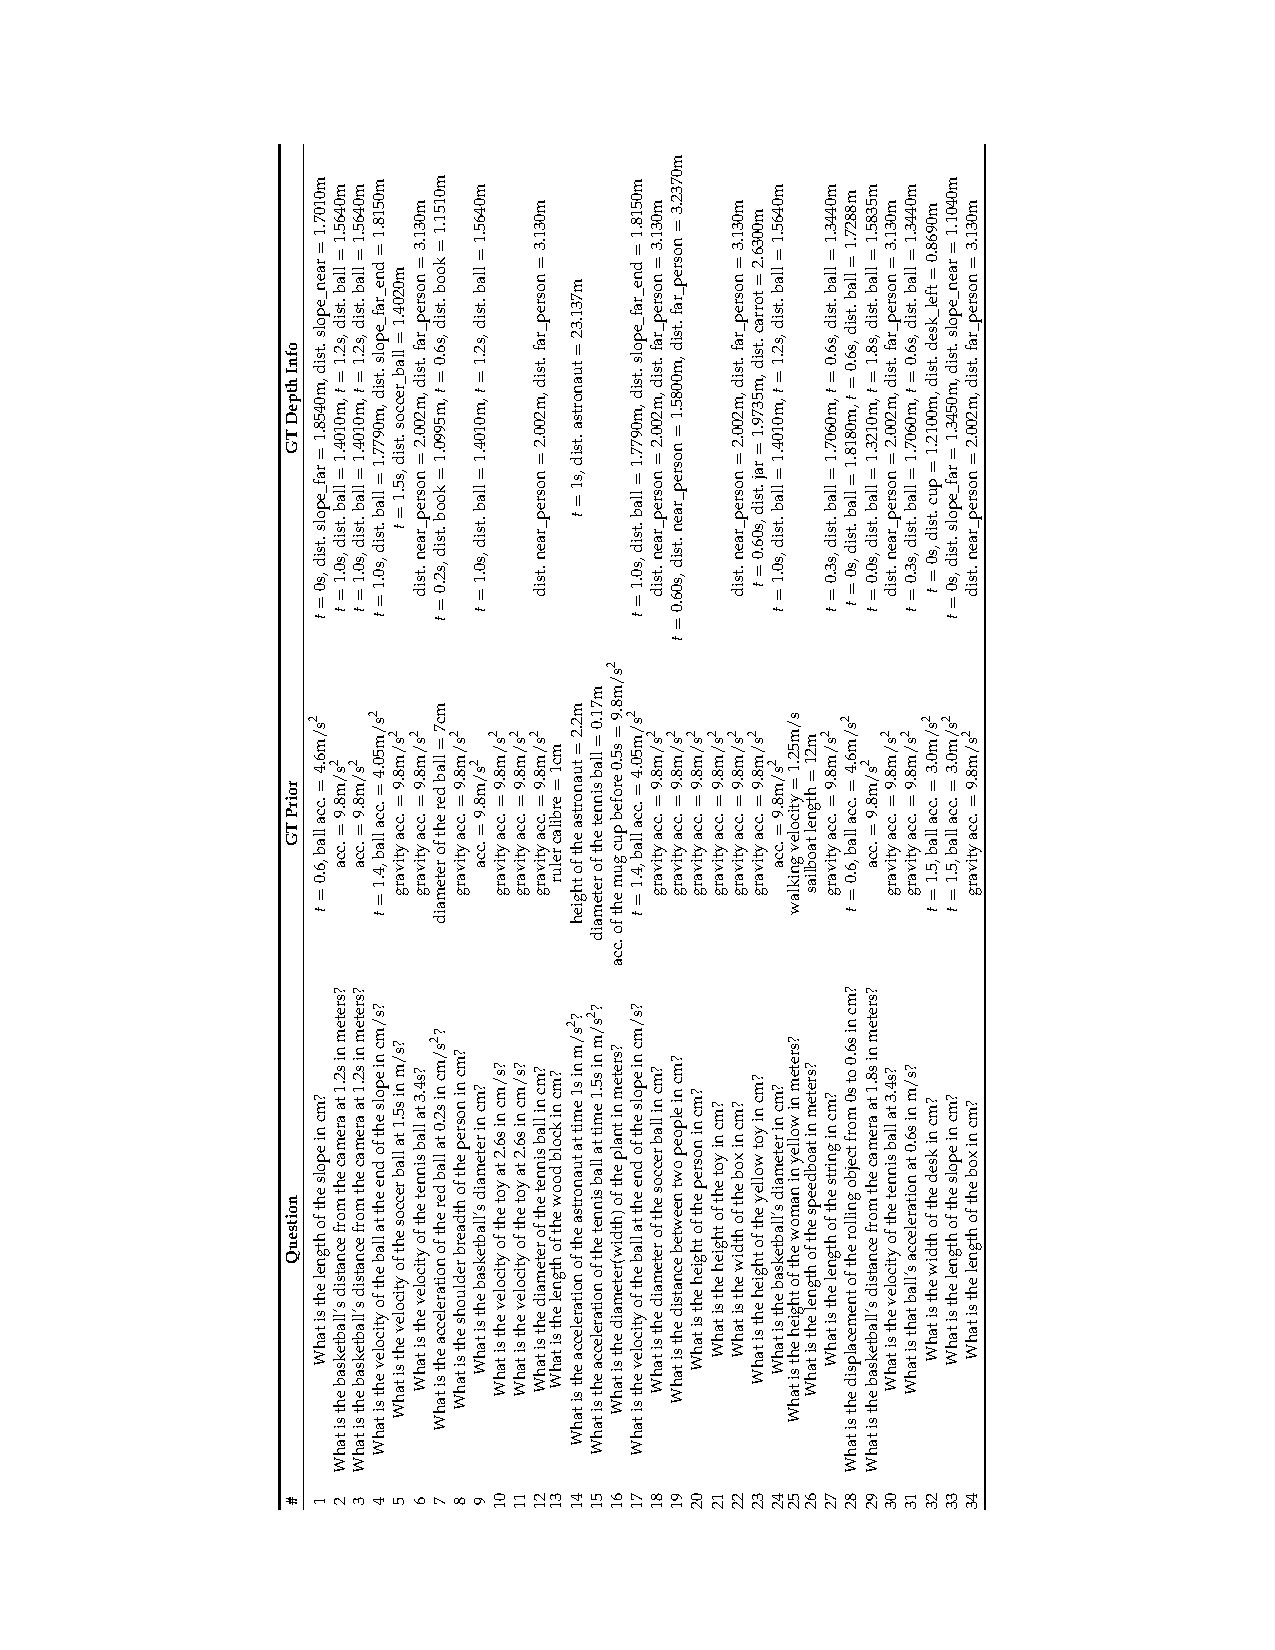
\includegraphics[width=.88\linewidth]{sec/images/parsing-examples1.pdf}
    \caption{\textbf{Selected examples of text inputs and answers (part 1).} Question is the natural-language prompt presented to the VLM. GT Prior is the physical prior provided to the model. GT Depth Info is the depth annotation used for \texttt{3D} reasoning tasks. GT Posterior is the numeric ground-truth answer to the kinematic inference question. See \autoref{tab:record-schema-example} for detailed explanation. Raw Response shows the corresponding VLM output for each model, and Parsed Value shows the parsed value extracted from the Raw Response.}
    \label{tab:parsing-examples1}
    \end{figure*}

\begin{figure*}[ht]
    \captionsetup{name=Table}
    \centering
    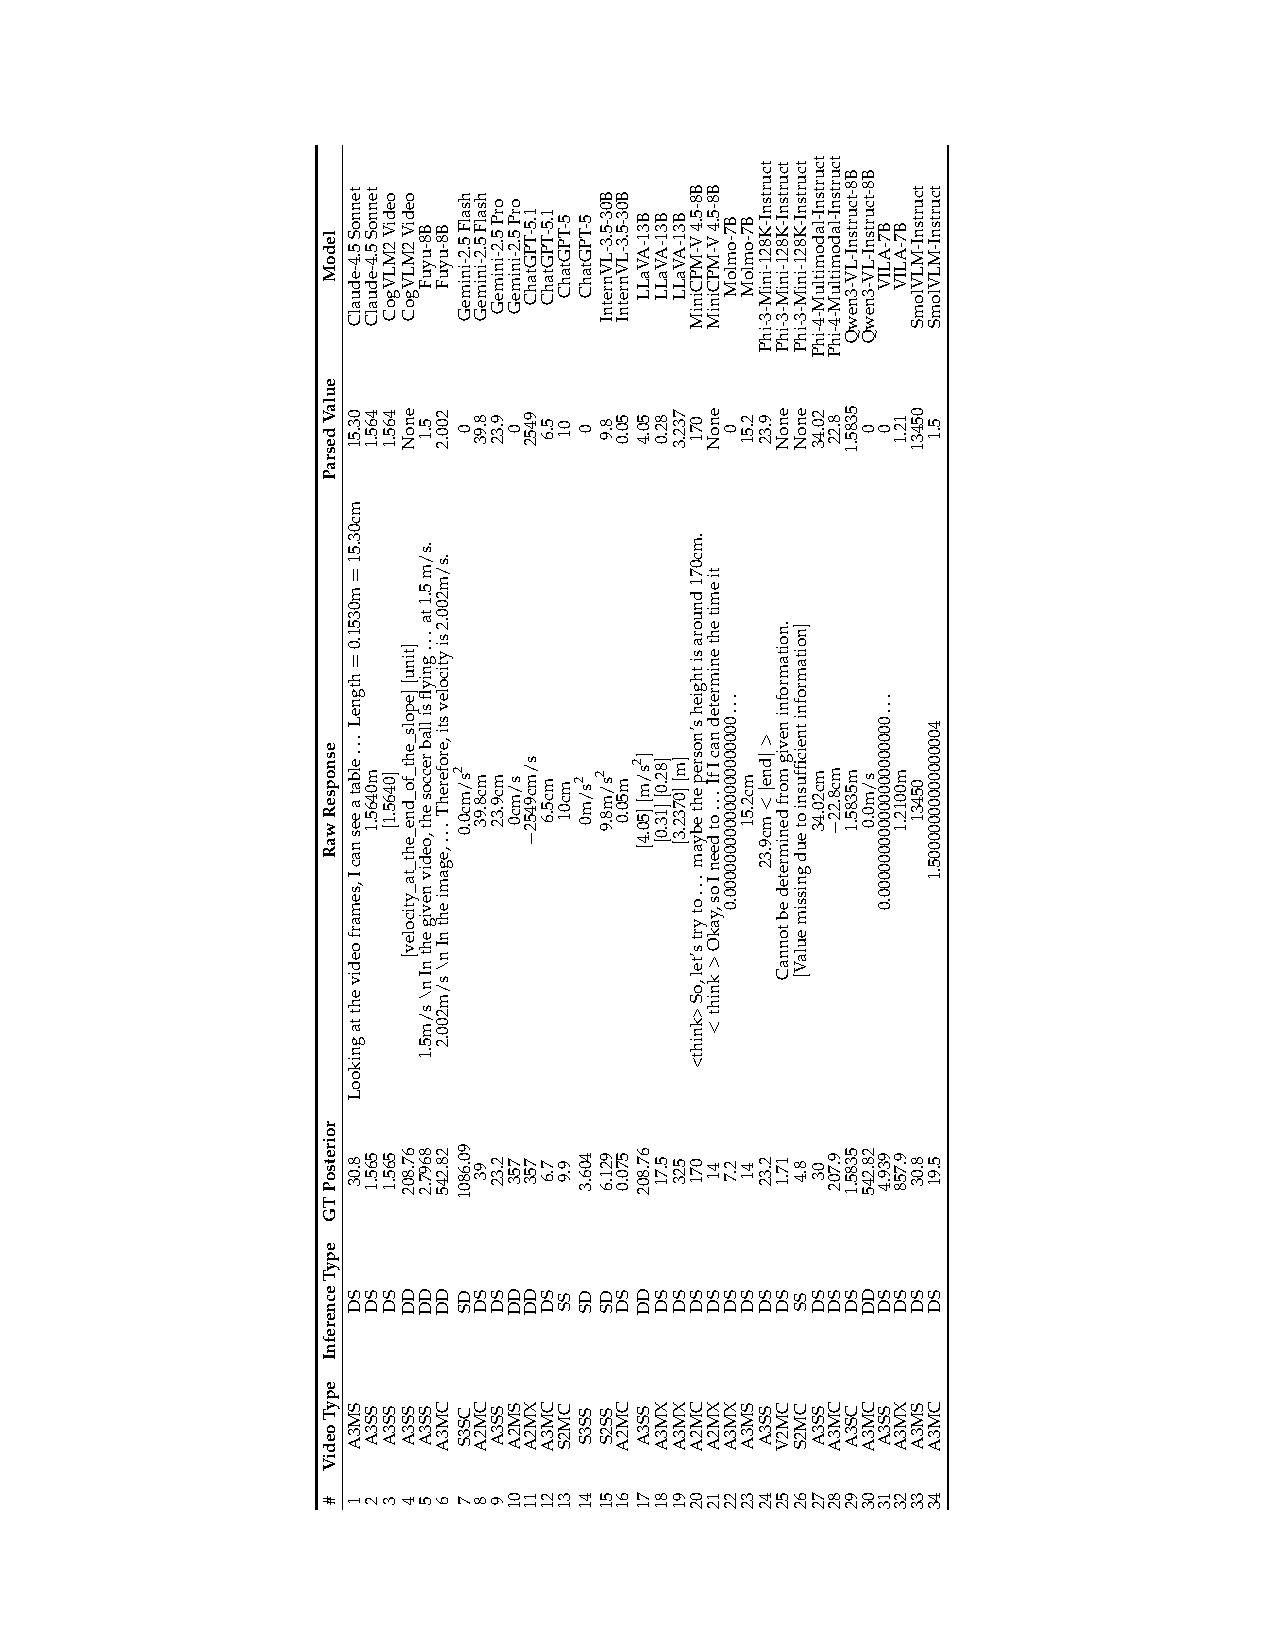
\includegraphics[width=.86\linewidth]{sec/images/parsing-examples2.pdf}
    \caption{\textbf{Selected examples of text inputs and answers (part 2).} Question is the natural-language prompt presented to the VLM. GT Prior is the physical prior provided to the model. GT Depth Info is the depth annotation used for \texttt{3D} reasoning tasks. GT Posterior is the numeric ground-truth answer to the kinematic inference question. See \autoref{tab:record-schema-example} for detailed explanation. Raw Response shows the corresponding VLM output for each model, and Parsed Value shows the parsed value extracted from the Raw Response.}
    \label{tab:parsing-examples2}
\end{figure*}

We evaluate a diverse suite of 21 VLMs, spanning proprietary closed-source APIs, open-source models hosted via Replicate, and open-source models deployed by our own.

\noindent \textbf{Proprietary Models.} We select flagship models from four major providers, including standard multimodal capabilities and those utilizing inference-time reasoning.

\begin{itemize}
    \item \textbf{OpenAI.} We evaluate two models: \textbf{GPT-5.1}~\cite{OpenAIgpt5.1} (\texttt{gpt-5.1-2025-11-13}) and \textbf{GPT-5}~\cite{OpenAIgpt5} (\texttt{gpt-5-2025-08-07}), both are flagship multimodal models. The latter is a ``thinking model'' that leverages Chain-of-Thought (CoT) processing for complex reasoning tasks. Both are accessed via the OpenAI API, accepting video inputs as sequences of base64-encoded frames to enable temporal understanding.
    
    \item \textbf{Google.} We evaluate \textbf{Gemini 2.5 Pro}~\cite{google2025gemini25pro} (\texttt{gemini-2.5-pro}), a high-capacity model capable of processing large context windows of interleaved images and text, and \textbf{Gemini 2.5 Flash}~\cite{google2025gemini25flash} (\texttt{gemini-2.5-flash}), a lightweight variant optimized for low-latency tasks. Both models accept base64 inline data and are optimized for complex reasoning across modalities.
    
    \item \textbf{Anthropic.} We utilize \textbf{Claude Sonnet 4.5}~\cite{anthropic2025claude45sonnet} (\texttt{claude-sonnet-4-5-20250929}). This model accepts a structured list of content blocks (text and base64-encoded images). It is characterized by its detailed explanatory capabilities, often providing extensive textual rationale alongside numerical answers. (See \autoref{tab:parsing-examples2} for raw response examples).

    \item \textbf{xAI.} We evaluate \textbf{Grok 4.1 (Fast Reasoning)}~\cite{xai2025grok41}, a model that combines rapid inference with advanced reasoning capabilities, designed to handle complex multimodal tasks with reduced latency while maintaining high accuracy.

\end{itemize}



\noindent \textbf{Open-source Models.} We also evaluate 15 distinct open-source models, representing a spectrum of architectures, parameter sizes, and input modalities to systematically assess architectural variations and scaling effects.

\begin{itemize}
    \item We include \textbf{LLaVA-13B}~\cite{liu2023visual}, a foundational baseline combining a Vicuna LLM with a CLIP encoder; \textbf{VILA-7B}~\cite{lin2023vila}, pre-trained on interleaved image-text data; and \textbf{Qwen3-VL-8B}~\cite{bai2025qwen25vl}, the latest iteration of Alibaba's vision-language series.
    
    \item To examine scaling effects across model sizes, we deploy and evaluate the \textbf{Qwen3-VL-Instruct} series at three scales: \textbf{2B}, \textbf{8B}, and \textbf{32B} parameters~\cite{bai2025qwen25vl}, enabling direct comparison of performance improvements with increased capacity within a single architecture family.

    \item Similarly, we assess the \textbf{InternVL-3.5} series across three parameter scales: \textbf{2B}, \textbf{8B}, and \textbf{30B}~\cite{chen2024internvl}, providing additional insights into how architectural choices interact with model scale for vision understanding.

    \item  We evaluate \textbf{Fuyu-8B}~\cite{adept2023fuyu}, which utilizes a simplified architecture processing raw image patches without a separate visual encoder.
    
    \item We test \textbf{Molmo-7B}~\cite{allenai2025molmo} and \textbf{SmolVLM}~\cite{marafioti2025smolvlm} (1.6B), both designed for high-efficiency reasoning on consumer hardware.
    
    \item \textbf{Phi-4 Multimodal}~\cite{microsoft2025phi4multi} and the smaller \textbf{Phi-3-Mini-128K-Instruct}~\cite{microsoft2024phi3}, both are Microsoft suite and process text interleaved with image lists.
    
    \item Finally, to assess temporal analysis capabilities, we include \textbf{MiniCPM-V 4.5}~\cite{yao2024minicpmv} and \textbf{CogVLM2-Video}~\cite{wang2024cogvlm2}. Distinct from frame-based approaches, these models accept direct video file inputs for native temporal processing.
\end{itemize}

In total, our evaluation encompasses \textbf{21 models} (6 proprietary and 15 open-source), providing comprehensive coverage of the current state-of-the-art in multimodal reasoning across different scales, architectures, and deployment paradigms.


\section{Prompt Design} \label{appendix:prompt_design}
For quantitative evaluation, we use a constrained generation strategy designed for precise numerical outputs. The system prompt explicitly restricts the output space, instructing the model to ``provide ONLY the numerical answer with units'' and emphasizing ``No explanation or reasoning needed.'' The prompt structure includes the visual input, system instructions, and ground truth priors and/or depth info, followed by the specific query and a post-prompt reinforcement. (See \autoref{fig:case1} for the Text Prompt template).

To ensure reproducibility, we enforce deterministic generation where possible. We set \texttt{temperature=0} (greedy decoding) for all models supporting this parameter. For hosted models via Replicate where explicit temperature control is unavailable, we utilize the default inference parameters recommended by the model maintainers.

The input sequence for all models is programmatically structured as \texttt{[Video Frames][System Prompt][Ground Truth Prior and/or Depth Info][Question][Post-prompt]}. Detailed examples are provided in \autoref{tab:parsing-examples1}.

\begin{itemize}
    \item \texttt{[Video Frames]}. This segment contains the full sequence of frames extracted from the source video, base64-encoded. We normalize all videos to 480p resolution. Our preliminary exploration indicated that while lower spatial resolution (480p) has negligible impact on physics reasoning, temporal subsampling (dropping frames) significantly degrades the tracking of velocity and acceleration. Therefore, we prioritize {temporal fidelity} by retaining all frames from the source video. This approach also distinguishes our methodology from most prior works, which often prioritize spatial resolution at the expense of frame rate.
    
    \item \texttt{[System Prompt]}. This serves as the behavioral instruction, establishing the persona that ``You are an expert video analyst...'' We selected this formulation following a pilot study of five prompt variations on a subset of 15 videos, which revealed no significant difference and this persona yielded the relatively highest adherence to formatting constraints without altering reasoning accuracy.
    
    \item \texttt{[Ground Truth Prior and/or Depth Info]}. This includes physical constants and contextual priors (e.g., ``Given that acceleration $a = 9.8 m/s^2$''). For \texttt{3D} scenes, this also includes depth information (e.g., ``At $t=1.0s$, the distance of the ball to the camera is $1.779m$...'') for estimation.
    
    \item \texttt{[Question]}. The specific physics query (e.g., ``What is the total displacement in the y-axis?'').
    
    \item \texttt{[Post-prompt]}. A final instruction reinforcing the output format (e.g., ``Provide... ONLY the numerical answer with units'') to mitigate the tendency of models to generate verbose "Chain-of-Thought" explanations in the final output.
\end{itemize}

\section{Answer Retrieval and Parsing} \label{sec:parsing}

For each question, we query the model once. To ensure robustness against API instability or transient errors, we implement an automated retry mechanism: if a query fails (e.g., timeout or server error) or yields a non-parsable response, the request is re-submitted up to a maximum of five times.

To extract quantitative data from potentially noisy model outputs, we employ a hierarchical parsing function (\texttt{parse\_number}) designed to handle both concise and verbose responses. The logic proceeds as follows.

\begin{enumerate}
    \item \textbf{Exact Match Validation:} We first check if the raw response strictly matches a numerical format (with or without units). If the response is concise (containing only a value and a unit matching the requested physical quantity), the numerical value is extracted directly.
    
    \item \textbf{Delimiter Search:} If the response is verbose, we scan for explicit answer markers, including \texttt{``="}, \texttt{``Final Answer:"}, \texttt{``Answer:"}, \texttt{``=>"}, and \texttt{``:"}. If a delimiter is identified, we discard the preceding text and retain only the substring immediately following it. If multiple cases are shown, we take the last occurrence. 
    
    \item \textbf{Unit Sanitization:} The retained text is cleaned of common physical units (e.g., ``meters'', ``m/s'', ``kg'') to prevent string processing errors during numerical extraction.
    
    \item \textbf{Heuristic Extraction:} Finally, a regular expression is applied to the cleaned text to identify floating-point numbers. We also take absolute value of the numerical answer. Crucially, if multiple numbers are found, we extract the {last} valid number in the sequence. This heuristic assumes that in verbose Chain-of-Thought responses, the final conclusion is located at the end of the text.
    
    \item \textbf{Failure Handling:} If no valid number is identified after these steps, the response is recorded as a failure (parsed as \texttt{None}).
\end{enumerate}

This strict parsing pipeline is essential because our evaluation metric relies on exact numerical regression. If a model provides only a qualitative description (e.g., ``The ball is moving quickly'', ``Cannot be determined'', or API error) or fails to reach a numerical conclusion within the decoding limit, it is then treated as a failure.

While most models adhered to the format constraints (i.e., [number] [unit]), we observed that \textbf{Claude Sonnet 4.5}, \textbf{Fuyu-8B}, and \textbf{MiniCPM-V 4.5} frequently generated verbose, multi-sentence explanations despite instructions to the contrary. By targeting the post-delimiter text and the last numerical value, our parsing logic effectively retrieves the correct answer from these verbose outputs. Representative examples of raw responses and their parsed values are detailed in \autoref{tab:parsing-examples2}.





